\begin{frame}{Ensembling}
\begin{itemize}
    \item No single model is perfect. Different models make different types of errors.
    \item Let's visualize the predictions of two different models:
\end{itemize}
\begin{figure}
    \centering
    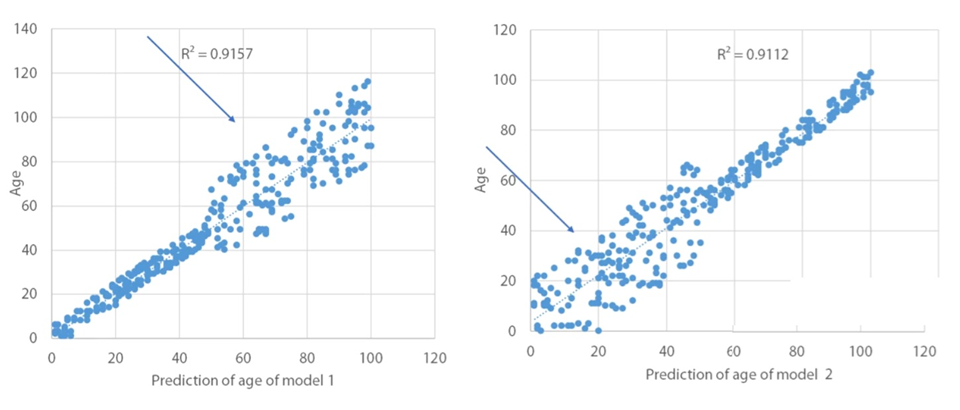
\includegraphics[width=1.0\linewidth]{images/ensembling1.png} 
    \caption{Predictions of Model 1 and Model 2}
\end{figure}
\end{frame}

\begin{frame}{Ensembling}
\begin{itemize}
    \item Combining predictions of diverse models can reduce errors and improve accuracy. This technique is called \textbf{Ensembling}.
\end{itemize}
\begin{figure}
    \centering
    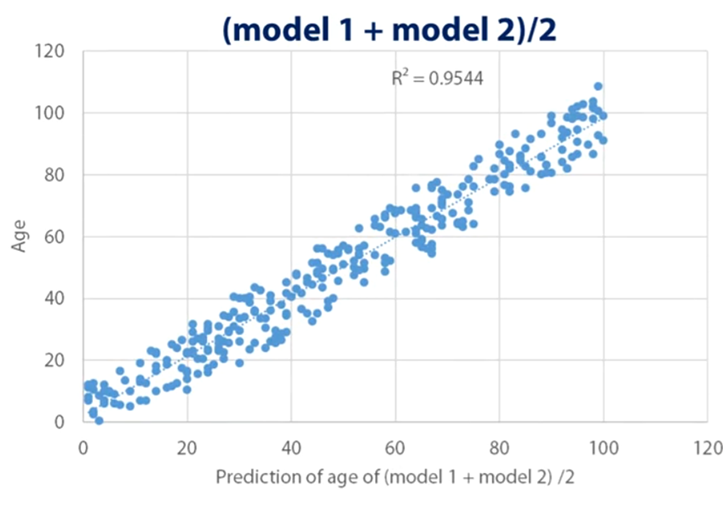
\includegraphics[width=0.7\linewidth]{images/ensembling2.png} 
    \caption{Averaged Predictions: Better Correlation}
\end{figure}
\end{frame}

\begin{frame}{Ensembling}
\begin{itemize}
    \item Diverse models are key to effective ensembling. Here are two strategies:
    \begin{itemize}
        \item \textbf{Bagging (Bootstrap Aggregating):} Train multiple models on different subsets of data (e.g., Random Forest model).
    \end{itemize}
    \end{itemize}
    \begin{figure}
    \centering
    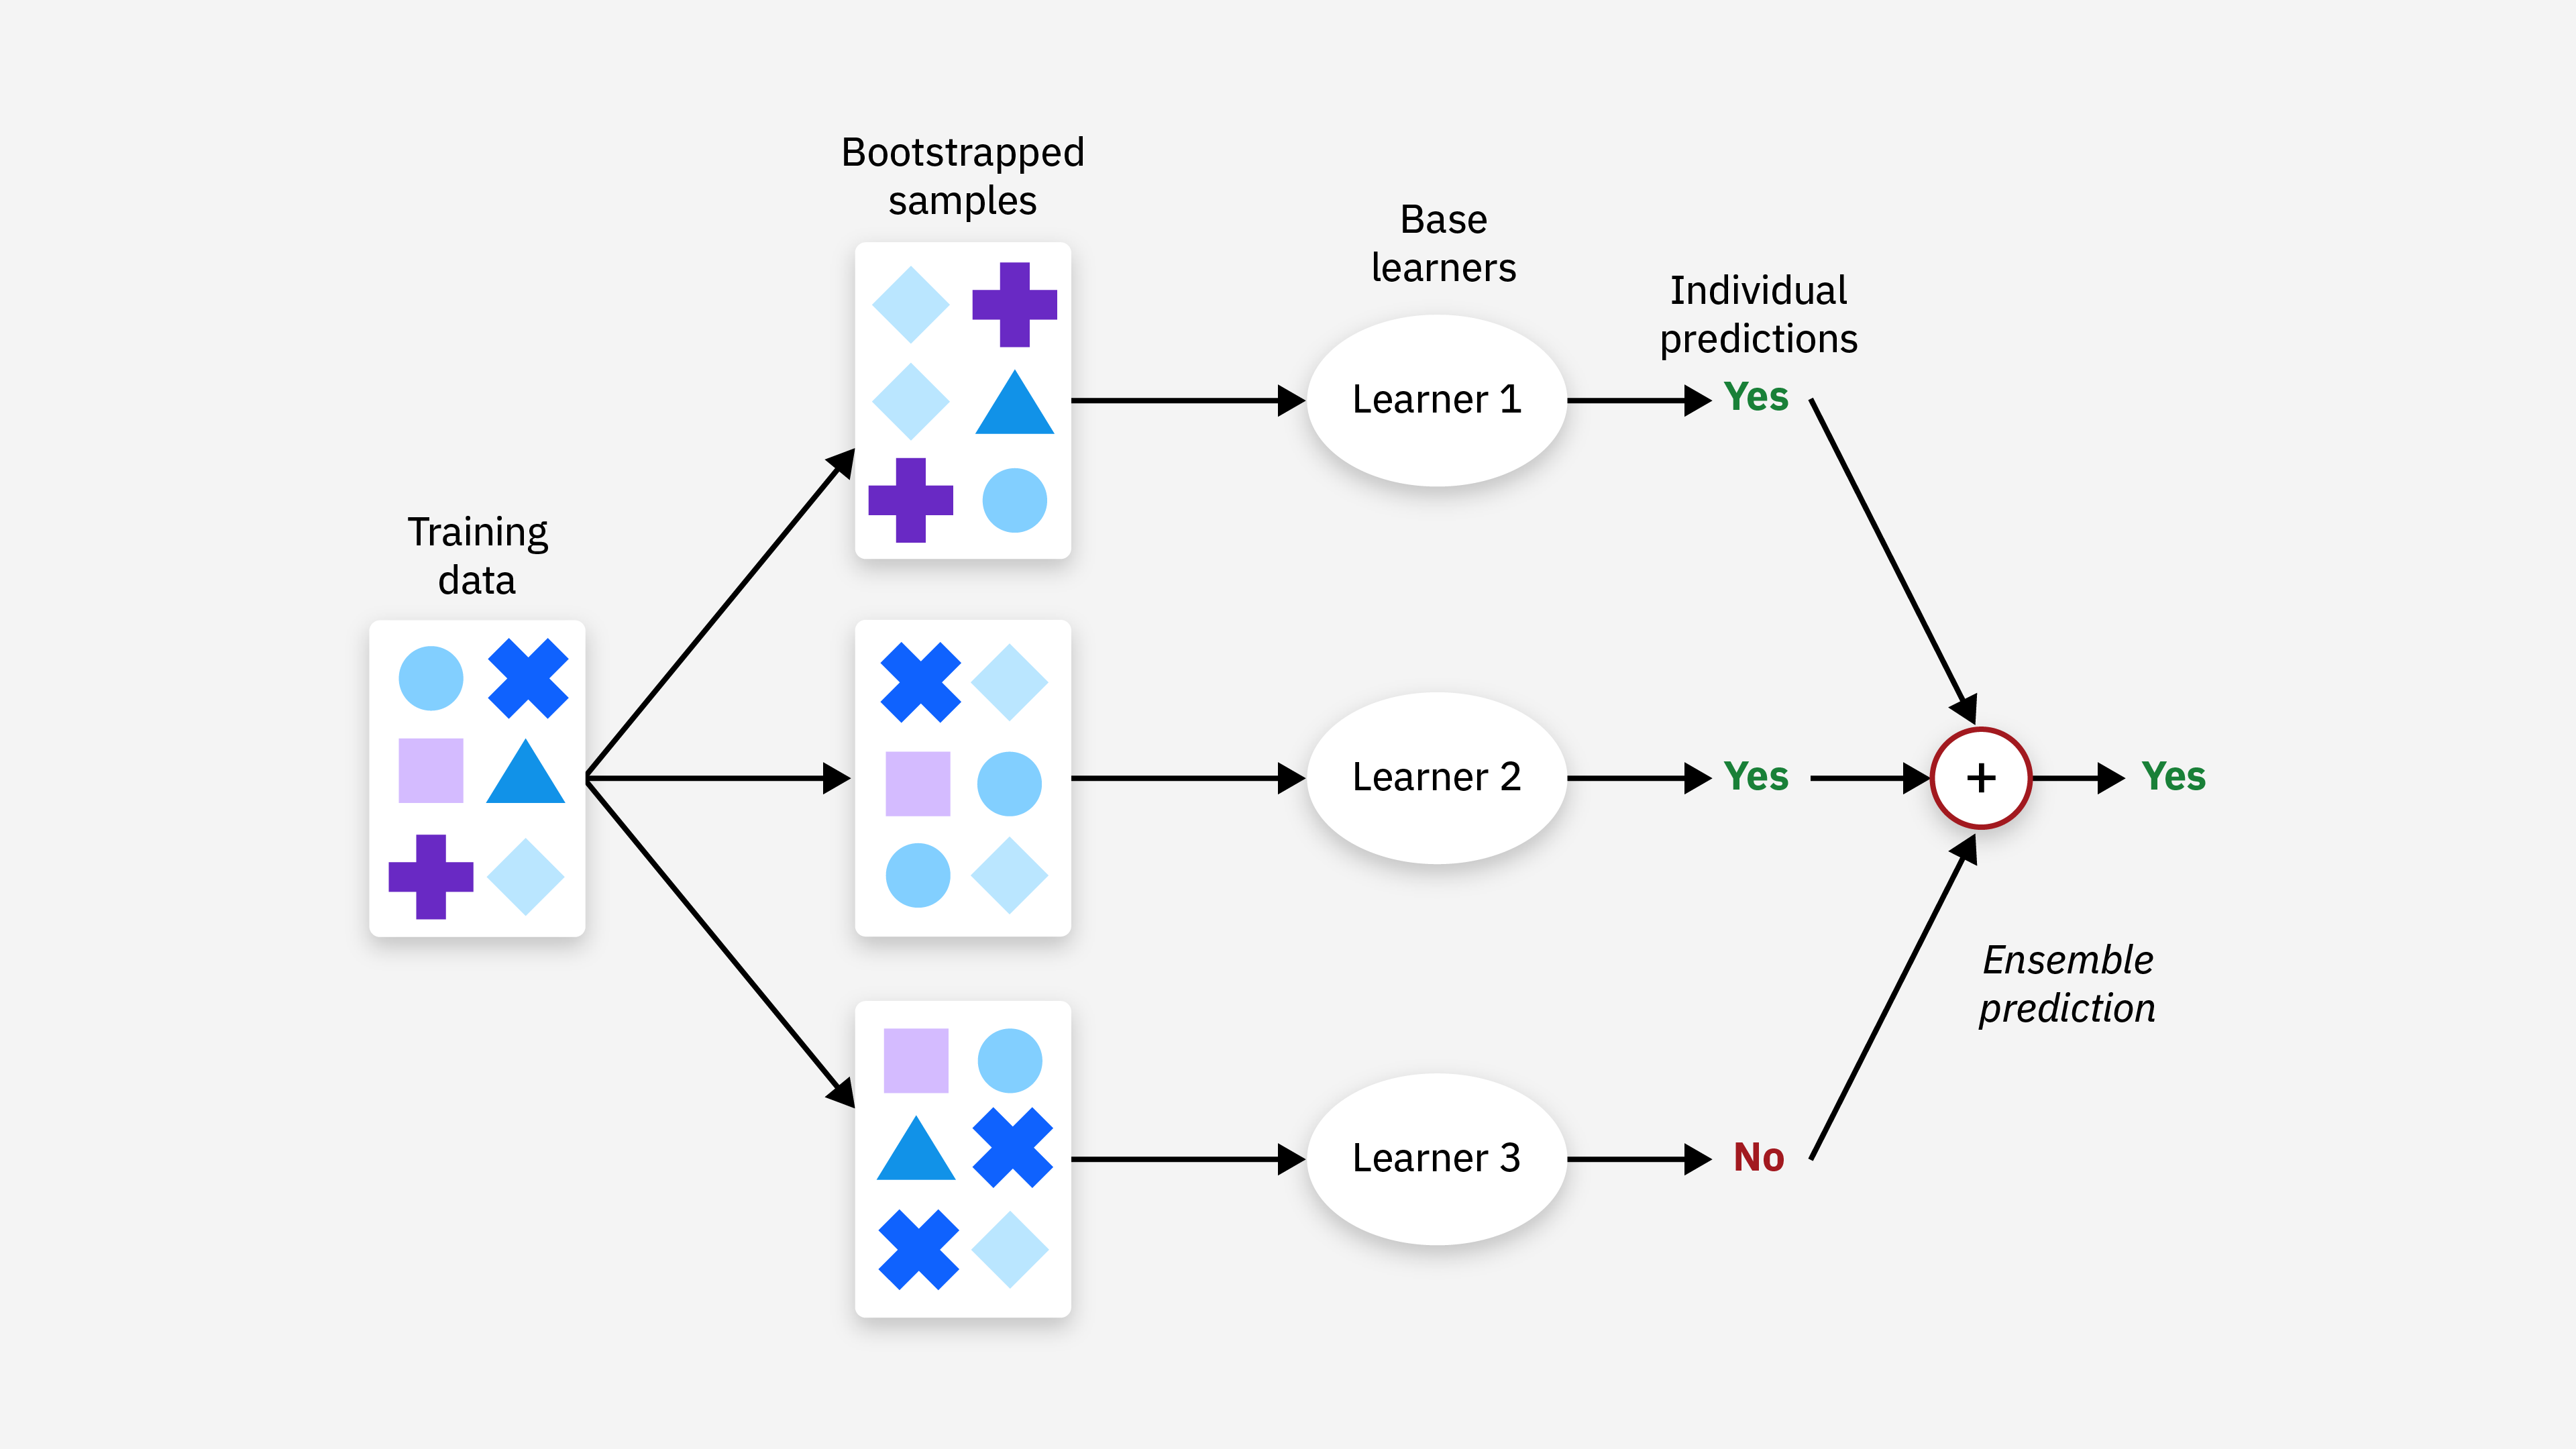
\includegraphics[width=0.8\textwidth,height=0.8\textheight,keepaspectratio]{images/bagging.png}
    \caption{Bagging example}
\end{figure}
\end{frame}

\begin{frame}{Ensembling}
\begin{itemize}
    \item Boosting:
    \begin{itemize}
        \item Train models sequentially, where each model focuses on the errors of the previous one (e.g., AdaBoost, Gradient Boosting).
    \end{itemize}
\end{itemize}
\begin{figure}
    \centering
    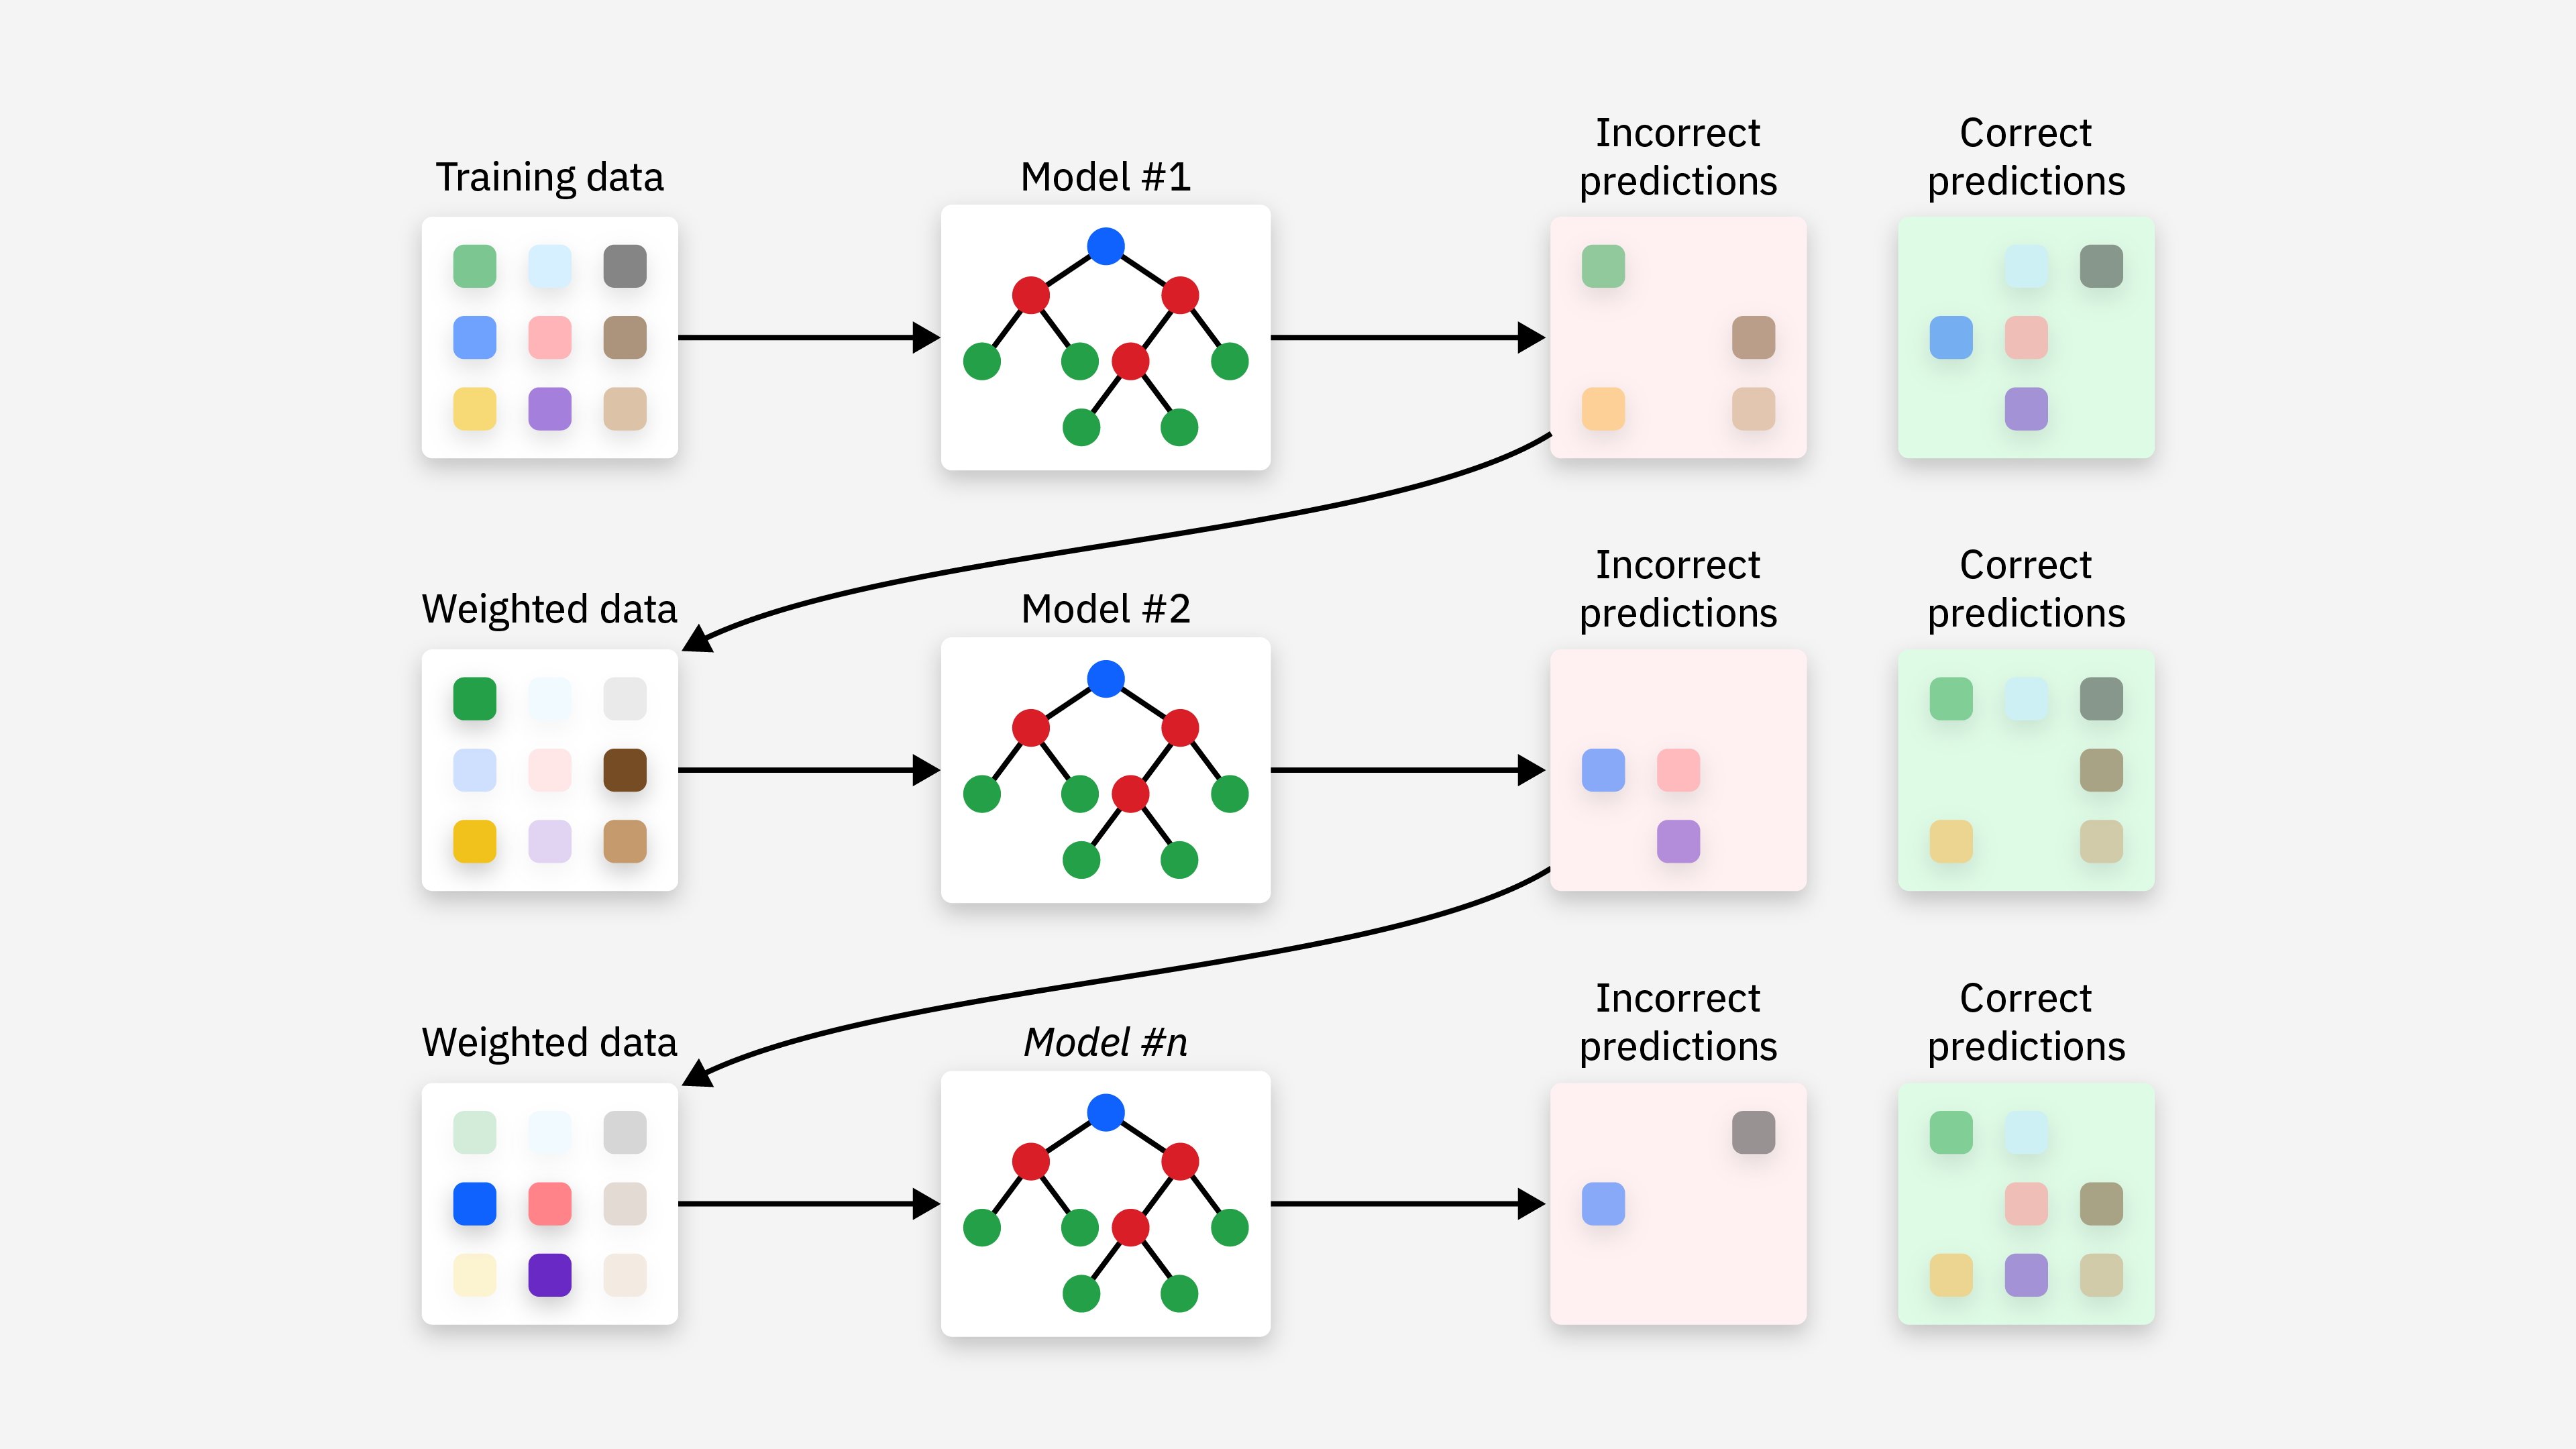
\includegraphics[width=0.8\textwidth,height=0.8\textheight,keepaspectratio]{images/boosting.png}
    \caption{Boosting Example}
\end{figure}
\end{frame}

\begin{frame}{Ensembling}
\begin{itemize}
\item These stratigies introduce diversity in models, but how can we combine their predictions?
\end{itemize}
\end{frame}

\begin{frame}{Ensembling}
\begin{itemize}
\item We can combine classifiers predictions using two ways:
\begin{itemize}
    \item \textbf{Hard Voting:}
    \begin{itemize}
        \item Each model votes for a class.
        \item The class with the majority of votes is selected.
    \end{itemize}
    \item \textbf{Soft Voting:}
    \begin{itemize}
        \item Average the predicted probabilities from each model.
        \item The class with the highest average probability is selected.
    \end{itemize}
\end{itemize}
\end{itemize}
\begin{figure}
    \centering
    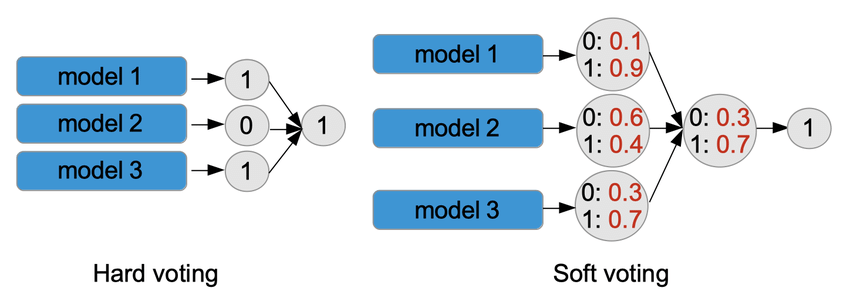
\includegraphics[width=0.8\linewidth]{images/voting.png}
    \caption{Illustration of Hard and Soft Voting for Classifiers}
\end{figure}
\end{frame}

\begin{frame}{Ensembling}
\begin{itemize}
\item We can combine classifiers predictions using two ways:
\begin{itemize}
    \item \textbf{Hard Voting:}
    \begin{itemize}
        \item Each model votes for a class.
        \item The class with the majority of votes is selected.
    \end{itemize}
    \item \textbf{Soft Voting:}
    \begin{itemize}
        \item Average the predicted probabilities from each model.
        \item The class with the highest average probability is selected.
    \end{itemize}
\end{itemize}
\end{itemize}
\begin{itemize}
\item For regressors:
    \begin{itemize}
        \item Take the average of predictions from all models.
        \end{itemize}
\end{itemize}
\end{frame}

\begin{frame}{Ensembling}
    \begin{itemize}
        \item Team-work is the best policy.
        \item We can train multiple networks for the same task then ensemble to get better results.
    \end{itemize}
\end{frame}

\begin{frame}{Ensembling - A simple Analysis}
    \begin{itemize}
        \item Let's assume that we have a test dataset with $N$ elements and an ensemble of $M$ models.
        \item Also assume that the probability of error of the label for an image on a model in the ensemble is denoted by $p(e)$ and is Independent and Identically Distributed (i.i.d)
        \item For an example assume $M=3$ and $e =0.01$
        \item Then probability of error of label for the max voting ensemble will be
        $$p(e) = 1 - (1-e)^3 - \binom 32 (1-e)^2 e$$
        \item For the above example $p(e)=0.0003$, which is significantly lower than a single model
    \end{itemize}
\end{frame} 